%% LyX 2.3.7 created this file.  For more info, see http://www.lyx.org/.
%% Do not edit unless you really know what you are doing.
\documentclass[aspectratio=169]{beamer}
\usepackage{lmodern}
\renewcommand{\sfdefault}{lmss}
\renewcommand{\ttdefault}{lmtt}
\usepackage[T1]{fontenc}
\usepackage[utf8]{inputenc}
\setlength{\parindent}{0cm}
\usepackage[active]{srcltx}
\usepackage{amssymb}
\usepackage{graphicx}
\ifx\hypersetup\undefined
  \AtBeginDocument{%
    \hypersetup{unicode=true}
  }
\else
  \hypersetup{unicode=true}
\fi

\makeatletter

%%%%%%%%%%%%%%%%%%%%%%%%%%%%%% LyX specific LaTeX commands.
%% A simple dot to overcome graphicx limitations
\newcommand{\lyxdot}{.}


%%%%%%%%%%%%%%%%%%%%%%%%%%%%%% Textclass specific LaTeX commands.
% this default might be overridden by plain title style
\newcommand\makebeamertitle{\frame{\maketitle}}%
% (ERT) argument for the TOC
\AtBeginDocument{%
  \let\origtableofcontents=\tableofcontents
  \def\tableofcontents{\@ifnextchar[{\origtableofcontents}{\gobbletableofcontents}}
  \def\gobbletableofcontents#1{\origtableofcontents}
}

%%%%%%%%%%%%%%%%%%%%%%%%%%%%%% User specified LaTeX commands.
%\usetheme{Warsaw}
%\usetheme{Pittsburgh}
\usetheme{Oxygen}
% or ...

%\setbeamercovered{transparent}
%\setbeamertemplate{headline}{}

\setbeamercovered{dynamic}
\setbeamertemplate{navigation symbols}{}


\definecolor{blue}{RGB}{0,102,255}
\definecolor{Babyblue}{rgb}{0.54, 0.81, 0.94}
\definecolor{mainblue}{RGB}{51, 51, 178}

\usepackage{color, colortbl}
\usepackage{xcolor}
\usepackage[utf8]{inputenc}

\usepackage{movie15}
\usepackage{animate}
\usepackage{graphicx}

\usepackage{array}
\usepackage{booktabs}
\usepackage{amssymb}
\usepackage{svg}
\usepackage{media9}
\usepackage{ulem}
\usepackage{amssymb}
\usepackage{pifont}

\usepackage[edges]{forest} 
\usepackage{tikz}
\usepackage{tikz-qtree}

%
\usepackage{tabularx}
\usepackage{etoolbox}
\usepackage{array}
\usepackage{colortbl}
\usepackage{longtable}
\usepackage{lscape}
\usepackage{multirow}
\usepackage{array}
\usepackage{arydshln}
\usepackage{bm}
%


\usepackage{forest}
\forestset{
  qtree/.style={
    baseline,
    for tree={
      parent anchor=south,
      child anchor=north,
      align=center,
      inner sep=1pt,
    }}}
\usepackage{flexisym}


%\renewcommand\makebeamertitle{{\logo{\includegraphics[width=4cm]{assets/EscudoUN-2016_styledv2.png}\vspace{0.75cm}}\maketitle}}
\renewcommand\makebeamertitle{{
	\setbeamertemplate{headline}{} 
	\setbeamertemplate{footline}{} 
	\begin{frame}{} 
		\vspace{0cm}     
		\titlepage
	\end{frame}
}}


\newcommand\ungraphic{{
	\vspace{-0.5cm}
	\includegraphics[width=0.1\textwidth]{assets/EscudoUN.png}\\
	\scriptsize{
		Universidad Nacional de Colombia\\
		Signal Processing and Recognition Group - SPRG\\
		Manizales, Colombia\\
		\today
	}
}}


\definecolor{UN_primary}{RGB}{148,180,59}
\definecolor{UN_comp4}{RGB}{177,178,176}

\makeatother


\begin{document}
\title{}
\title[Developing an AI-Driven Framework for Real-Time Signal Processing
and Data Management]{Developing an AI-Driven Framework for\\Real-Time Signal Processing
and Data Exchange}
\author{Yeison Nolberto Cardona-Álvarez}
\institute{\textbf{Advisor:} Andres Marino Alvarez-Meza, Ph.D\\
\textbf{Co-Advisor:} Germán Castellanos-Domínguez, Ph.D}
\titlegraphic{\ungraphic}
\date{}

\makebeamertitle

%% \AtBeginSection[]{\frame<beamer>{\frametitle{Outline}\tableofcontents[currentsection,currentsubsection]}}

\let\oldcite\cite
\renewcommand*\cite[1]{{\color {gray}\tiny{\oldcite{#1}}}}
\newcommand*\citet[1]{{\color {gray}\fontsize{4}{4}\selectfont{\oldcite{#1}}}}
\newcommand*\reallysmall[1]{{\color {gray}\fontsize{2}{2}\selectfont{\oldcite{#1}}}}

\begin{frame}{Outline}

\tableofcontents{}
\end{frame}

\section{Motivation}
\begin{frame}{Motivation}

\framesubtitle{Data Exchange: Definition}

Data Exchange refers to the \textbf{efficient and secure} flow of
data between different platforms and procedures \cite{zhang2021fault,thakare2021secure}.

\vfill{}

\begin{figure}
\centering{}\includegraphics[width=0.3\textwidth]{images/data_exchange_1}
\end{figure}
 

\end{frame}
%
\begin{frame}{Motivation}

\framesubtitle{Data Exchange: Applications and Investments}

It requires strong security and encryption, data quality and dependability,
and industry-specific \textbf{compliance standards} \cite{attiogbe2021advances}.
\begin{columns}[t]

\column[b]{0.66\textwidth}
\begin{itemize}
\item {\scriptsize{}Business intelligence and analytics \cite{kouper2021challenges}. }{\scriptsize\par}
\item {\scriptsize{}Finance and banking \cite{Elsaify2021Data}.}{\scriptsize\par}
\item {\scriptsize{}Government and public services \cite{Ball2020Organizational}.}{\scriptsize\par}
\item {\scriptsize{}Marketing and advertising \cite{mishra2023application}.}{\scriptsize\par}
\item {\scriptsize{}Healthcare \cite{al2022application}.}{\scriptsize\par}
\item {\scriptsize{}Research and academia \cite{qiu2021comprehensive,paltun2021diverse,adiga2022enhancing}.}{\scriptsize\par}
\end{itemize}

\column[b]{0.34\textwidth}

{\scriptsize{}}{\scriptsize\par}

\begin{figure}
\centering{}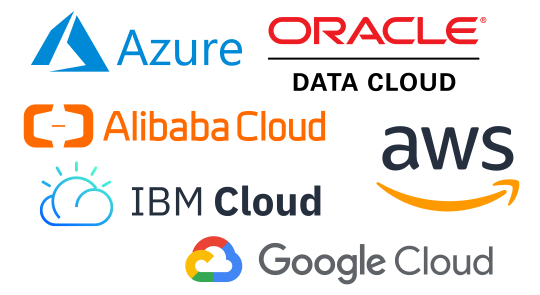
\includegraphics[width=1\columnwidth]{images/datacenters}
\end{figure}

\end{columns}

\end{frame}
%
\begin{frame}{Motivation}

\framesubtitle{The Growth of Data Centers in Colombia}

Latin America's technological revolution plays a crucial role in promoting
\textbf{regional economic growth}, closing the digital gap, creating
a foundation for improved connectivity, innovation, and robust digital
infrastructure \cite{KearneyGlobalServices2023}.
\begin{columns}[t]

\column[b]{0.6\textwidth }
\begin{itemize}
\item {\scriptsize{}Fourth largest data center market in Latin America.
}{\scriptsize\par}
\item {\scriptsize{}Significant investments in infrastructure. }{\scriptsize\par}
\item {\scriptsize{}Attractive for international investments. }{\scriptsize\par}
\item {\scriptsize{}Strategic location advantage. }{\scriptsize\par}
\end{itemize}

\column[b]{0.4\textwidth }

\begin{figure}
\centering{}\includegraphics[width=0.5\columnwidth]{images/platanal}
\end{figure}

\end{columns}

\end{frame}
%
\begin{frame}{Motivation}

\framesubtitle{AI-Driven Hyperautomation: The Future of Smart Workflows}

\textbf{Hyperautomation} elevates traditional software automation,
infusing it with AI to transform data ecosystems into adaptive, \textbf{self-optimizing
entities}, reshaping the dynamics of data management and analysis.
\begin{columns}[t]

\column{0.5\textwidth}
\begin{itemize}
\item {\scriptsize{}Data Process Automation }{\scriptsize\par}
\item {\scriptsize{}Analysis and Decision-Making }{\scriptsize\par}
\item {\scriptsize{}Workflow Optimization }{\scriptsize\par}
\item {\scriptsize{}System Integration }{\scriptsize\par}
\item {\scriptsize{}Data Governance }{\scriptsize\par}
\item {\scriptsize{}Scalability and Maintenance }{\scriptsize\par}
\end{itemize}

\column{0.5\textwidth}

\begin{figure}
\centering{}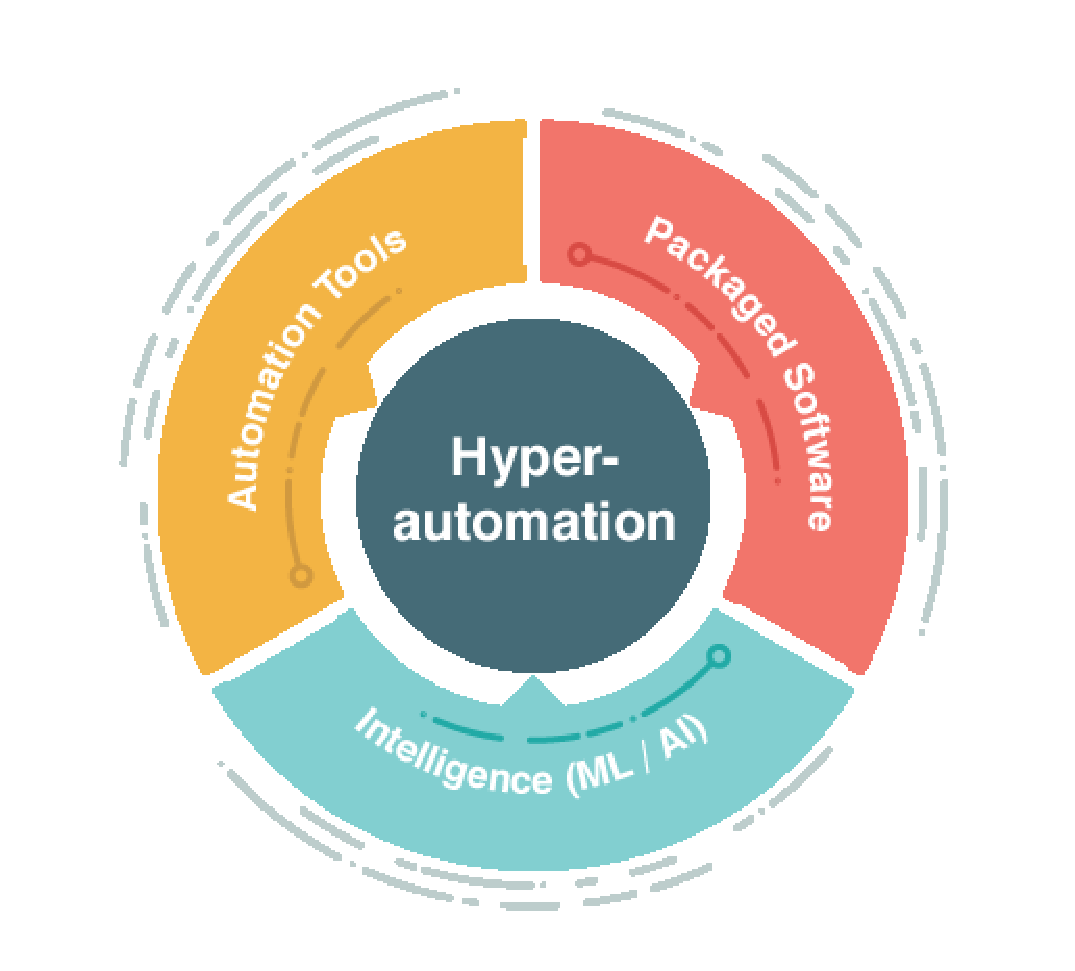
\includegraphics[width=0.5\columnwidth]{images/Hyperautomation-1}
\end{figure}

\end{columns}

\vfill{}
Integrating \textbf{AI} into software transforms data ecosystems into
intelligent, self-evolving networks, revolutionizing the approach
to data management and analysis. \cite{haleem2021hyperautomation}. 
\end{frame}
%
\begin{frame}{Motivation}

\framesubtitle{SPRG: Signal Processing and Recognition Group}

Our research group develops \textbf{transdisciplinary data exchange}
since we know that it exposes novel approaches and supports collaborative
discoveries \textbf{across academic areas} \cite{gomezestrategia,aguirre2023feet}.
\begin{columns}[t]

\column[b]{0.5\textwidth}
\begin{itemize}
\item {\scriptsize{}Data heterogeneity.}{\scriptsize\par}
\item {\scriptsize{}Handling unstructured data.}{\scriptsize\par}
\item {\scriptsize{}Real-Time Data Processing and Exchange.}{\scriptsize\par}
\item {\scriptsize{}Privacy and security regulations.}{\scriptsize\par}
\item {\scriptsize{}Interoperability and accessibility.}{\scriptsize\par}
\item {\scriptsize{}Scalability and efficient management.}{\scriptsize\par}
\end{itemize}

\column[b]{0.5\textwidth}

\begin{figure}
\centering{}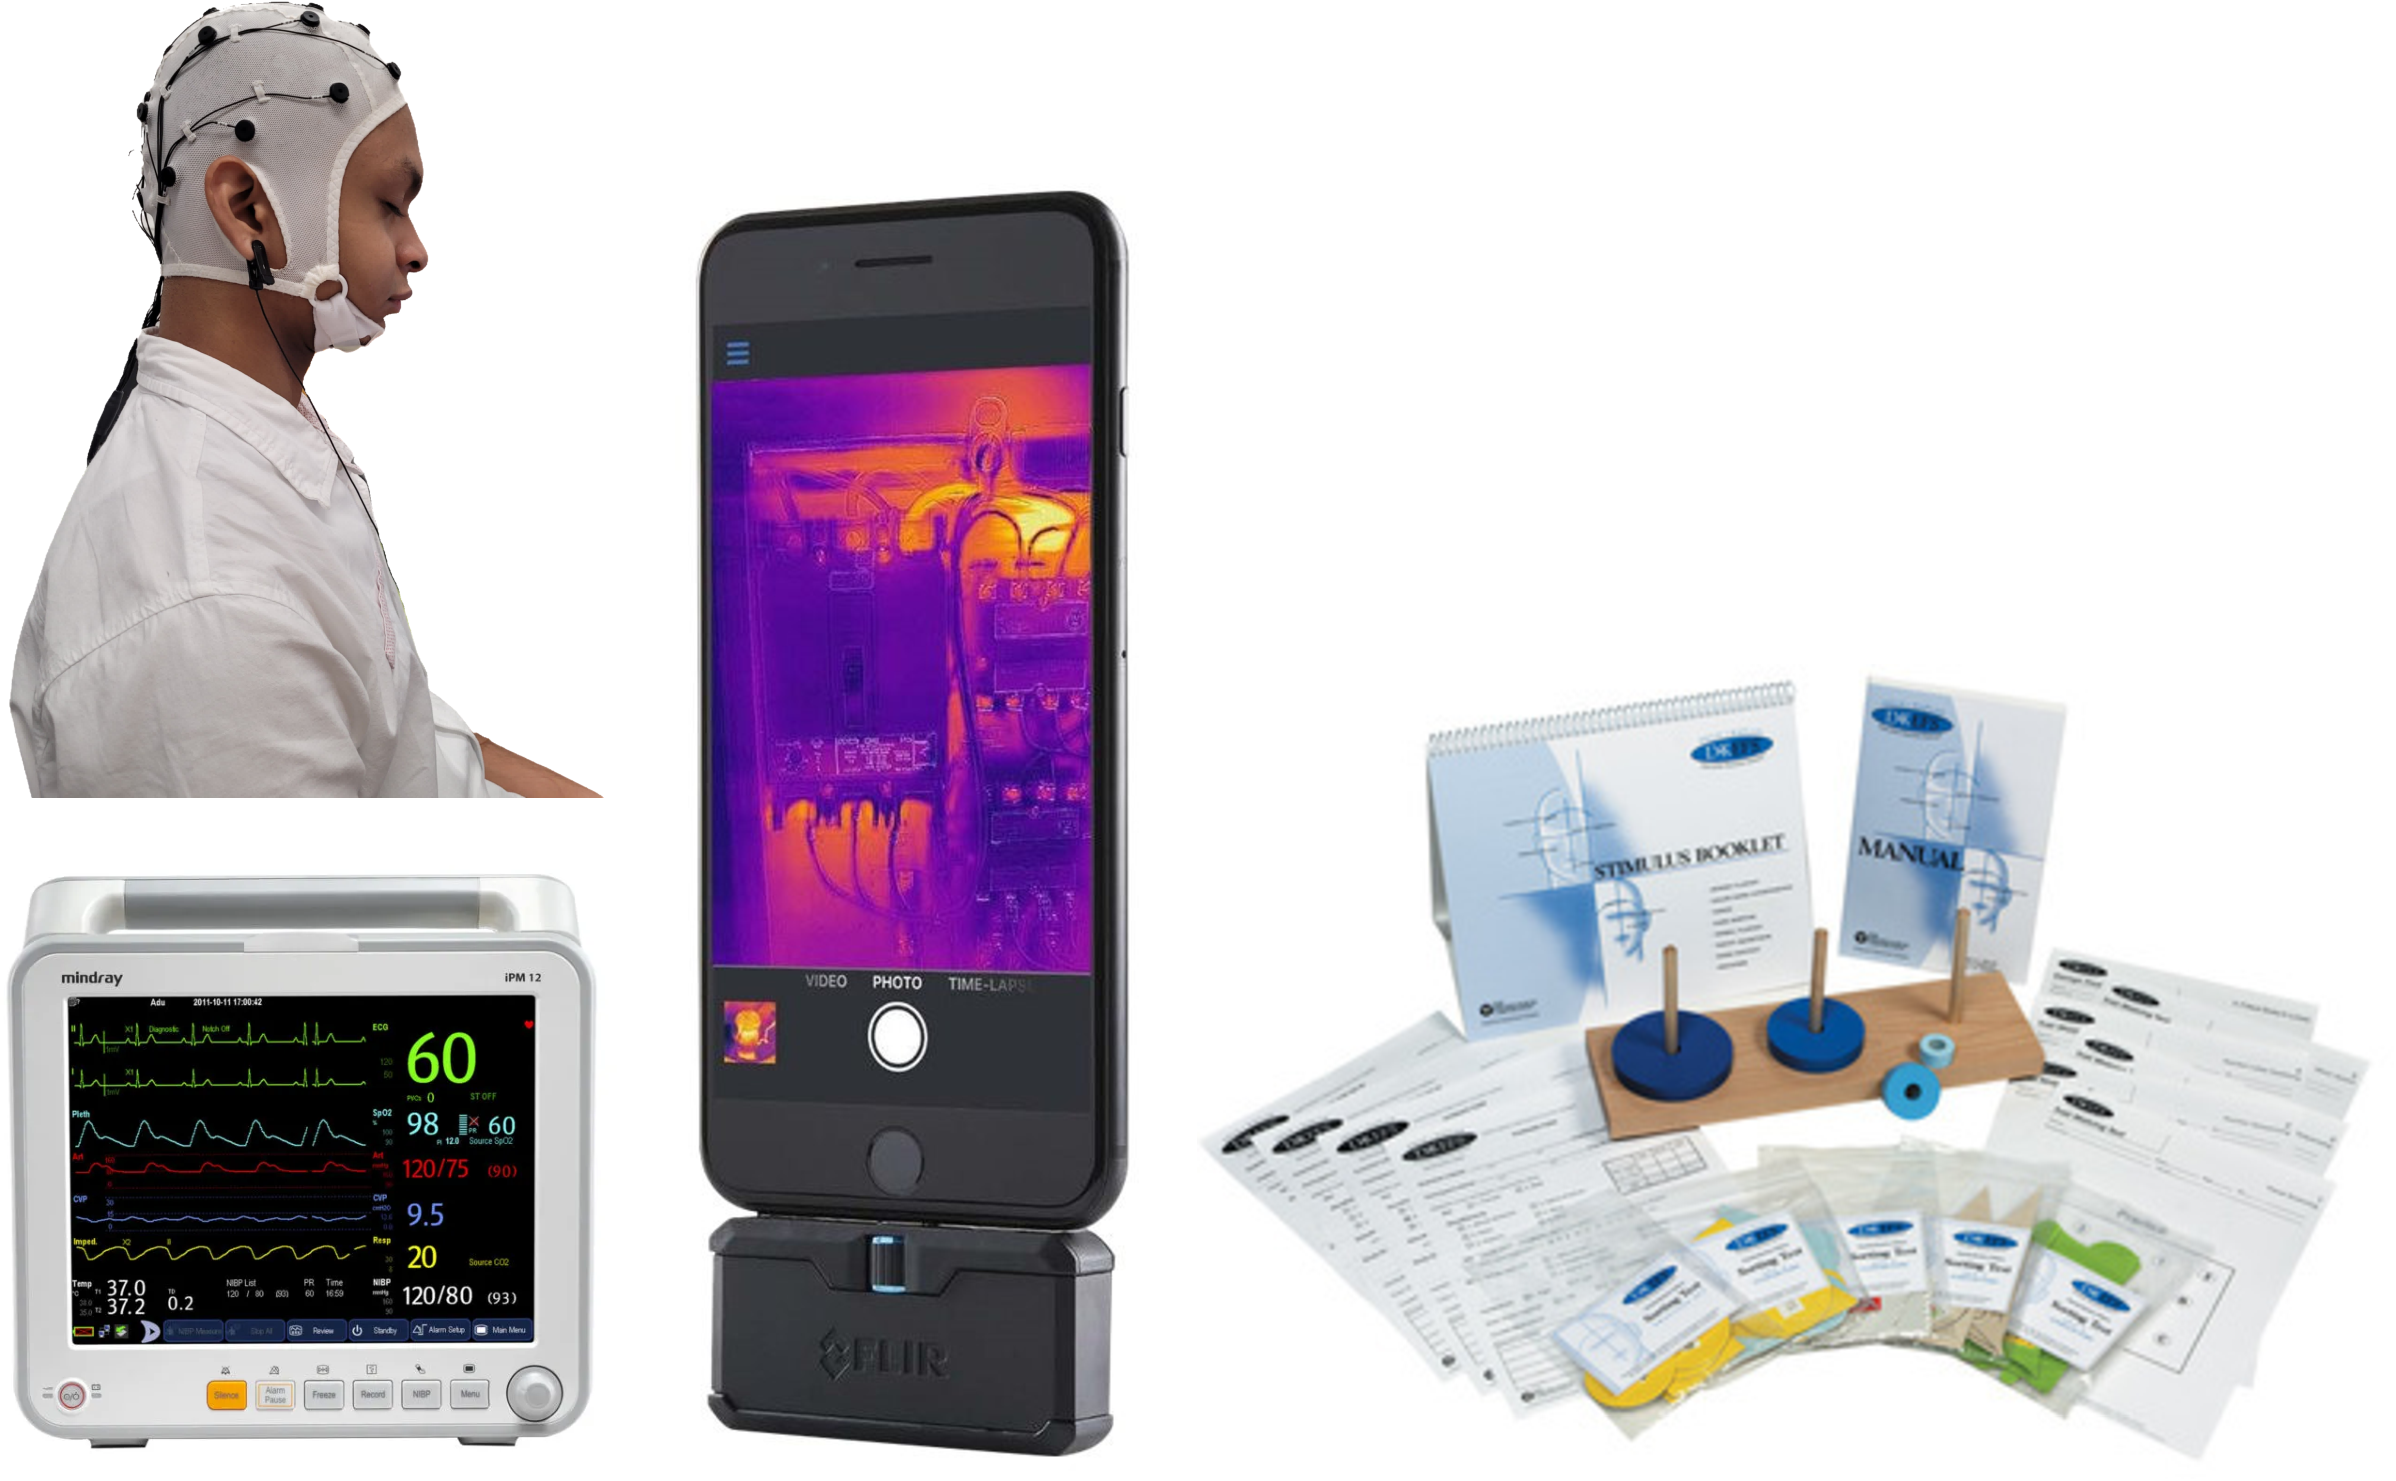
\includegraphics[width=1\columnwidth]{images/research}
\end{figure}

\end{columns}

\end{frame}

\section{Problem Statement}

\begin{frame}{Problem Satement}

\framesubtitle{Methodologies for Data Exchange }

 
\begin{columns}[t]

\column{0.5\textwidth}
\begin{description}
\item [{{\scriptsize{}APIs:}}] {\scriptsize{}They are limited by request
rate, security, and provider stability/changes \cite{velepucha2023survey}.}{\scriptsize\par}
\end{description}
\vspace{1cm}

\begin{description}
\item [{{\scriptsize{}Messaging:}}] {\scriptsize{}Scalability, delivery
assurance, state management, and security issues in distributed systems.
\cite{fang2019integrating}.}{\scriptsize\par}
\end{description}

\column{0.5\textwidth}
\begin{description}
\item [{{\scriptsize{}ETL:}}] {\scriptsize{}Performance and complexity
concerns related to data quality and handling large amounts of diverse
data. \cite{abdelhafiz2021sharding}.}{\scriptsize\par}
\end{description}
\vspace{1cm}

\begin{description}
\item [{{\scriptsize{}File\ Transfer:}}] {\scriptsize{}Security, file
size, and bandwidth issues \cite{ordonez2023blockchain,yi2023compound}.}{\scriptsize\par}
\end{description}
\end{columns}

\end{frame}
%
\begin{frame}{Problem Statement}

\framesubtitle{API Request Limits}

API request \textbf{rate limits} may cause data transmission difficulties,
especially in multimodal and real-time situations, and make API provider
changes \textbf{harder to adapt} and maintain \cite{Malki2022Impact,Malki2023Combining}.

\begin{figure}
\centering{}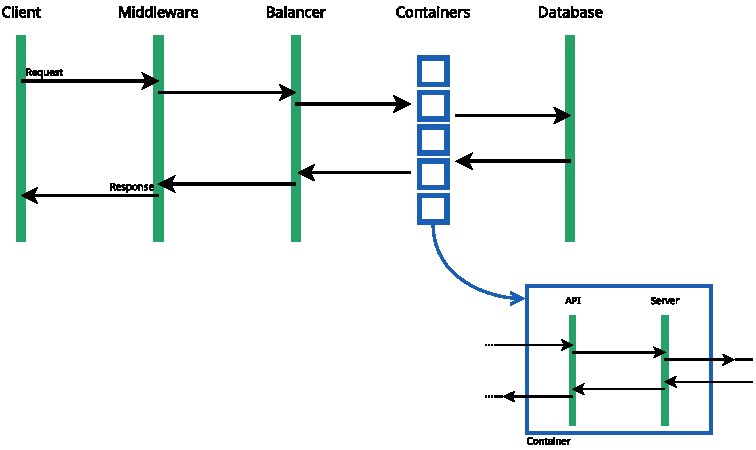
\includegraphics[height=0.35\paperheight]{images/diagrams/API_01}
\end{figure}

\begin{center}
\textsl{\textcolor{red}{\scriptsize{}Manual configurations limit API
effectiveness in multimodal and real-time environments.}}{\scriptsize\par}
\par\end{center}

\end{frame}
%
\begin{frame}{Problem Statement}

\framesubtitle{Messaging Scalability}

Scalability and delivery certainty problems in distributed messaging
systems can lead to the \textbf{loss or delay of messages}, which
can have a severe influence on the \textbf{efficiency and reliability}
of communication in real-time and multimodal contexts \cite{Arellanes2020Evaluating,basin2020scalable}.

\begin{figure}
\centering{}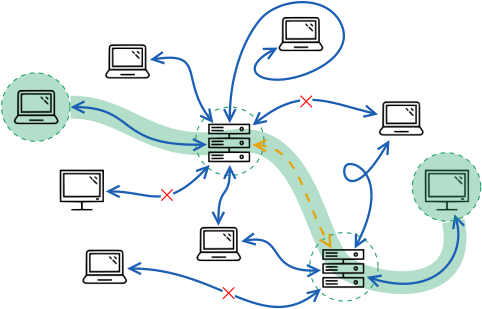
\includegraphics[height=0.35\paperheight]{images/diagrams/MSG_01}
\end{figure}

\begin{center}
\textsl{\textcolor{red}{\scriptsize{}Centralized server reliance in
distributed messaging often results in inefficient routing.}}{\scriptsize\par}
\par\end{center}

\end{frame}
%
\begin{frame}{Problem Statement}

\framesubtitle{Multimodal ETL \& AI }

Complex multimodal ETL processes can lead to \textbf{inaccurate data
and disruptions} in AI analysis due to challenges with data integration
and real-time data management

\cite{Qaiser2023Comparative,Soussi2021Big-Parallel-ETL:}.

\begin{figure}
\centering{}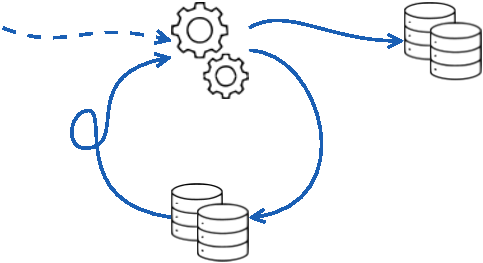
\includegraphics[height=0.35\paperheight]{images/diagrams/ETL_01}
\end{figure}

\begin{center}
\textsl{\textcolor{red}{\scriptsize{}Relying on rigid, sequential
data handling poses challenges in data integration and real-time management
.}}{\scriptsize\par}
\par\end{center}

\end{frame}
%
\begin{frame}{Problem Statement}

\framesubtitle{Large-Scale File Transmission}

 

Large-scale file transmission requires efficient and safe administration
of continuous data flow, especially in integrating systems and platforms,
while ensuring data \textbf{integrity} and \textbf{accessibility}
in changing contexts \cite{Zheng2020Design,yin2023network}.

\begin{figure}
\centering{}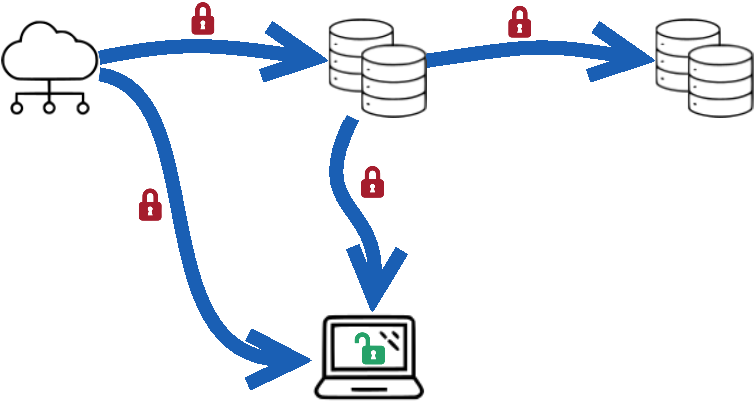
\includegraphics[height=0.35\paperheight]{images/diagrams/FLA_01}
\end{figure}

\begin{center}
\textsl{\textcolor{red}{\scriptsize{}Depends primarily on protocols
that are static and universally applicable.}}{\scriptsize\par}
\par\end{center}
\end{frame}

\section{State-of-the-Art}

\begin{frame}{State-of-the-Art}

\framesubtitle{APIs: Infrastructure Improving}

\noindent {\footnotesize{}}{\footnotesize\par}

\begin{forest}
  qtree,
  for tree={
    grow=0,             
    parent anchor=children,       
    child anchor=parent, 
    anchor=parent,
    l sep=5mm,  
	font=\tiny,       
  },
  where level=0{
    %grow=0,            
  }{
    if n children=0{folder}{}, 
    edge path'={(!u.parent anchor) -- ++(2.5mm,0) |- (.child anchor)[line width=0.6pt]},
  }
  [Optimization in\\Computer Systems, rotate=90 
    [Resource\\Management, rotate=90
      [Dynamic Resources Management Under Limited Communication Based on Multi-level Agent System \citet{wang2023dynamic}.]
      [Online Task Allocation and Scheduling in Fog IoT using Virtual Bidding \citet{joshi2022online}.]
    ]
    [Communication\\Efficiency, rotate=90 
      [Event-Triggered Communication Network with Limited-Bandwidth Constraint for Multi-Agent Reinforcement Learning \citet{hu2021event}.]
      [Adaptive REST API Testing with Reinforcement Learning \citet{kim2023adaptive}.]
    ]
    [Real-Time\\Systems, rotate=90  
      [On the Design and Implementation of Real-Time Resource Access Protocols \citet{dos2020design}.]
      [Towards Self-Managing Cloud Storage with Reinforcement Learning \citet{noel2019towards}.]
    ]
  ]
\end{forest}

\vfill{}

\begin{center}
\textsl{\textcolor{red}{\scriptsize{}Limitations in }}\textbf{\textsl{\textcolor{red}{\scriptsize{}real-time
API performance}}}\textsl{\textcolor{red}{\scriptsize{} and }}\textbf{\textsl{\textcolor{red}{\scriptsize{}adaptability}}}\textsl{\textcolor{red}{\scriptsize{}
due to static configuration settings.}}{\scriptsize\par}
\par\end{center}

\end{frame}
%
\begin{frame}{State-of-the-Art}

\framesubtitle{Distributed Messaging: Scalability and Reliability}

\begin{forest}
  qtree,
  for tree={
    grow=0,             
    parent anchor=children,       
    child anchor=parent, 
    anchor=parent,
    l sep=5mm,  
	font=\tiny,       
  },
  where level=0{
    %grow=0,            
  }{
    if n children=0{folder}{}, 
    edge path'={(!u.parent anchor) -- ++(2.5mm,0) |- (.child anchor)[line width=0.6pt]},
  }
  [Distributed Real-Time\\Messaging and Scalability, rotate=90 
    [Event Streaming and\\Async. Communication, rotate=90
      [Reliability enhancements for high-availability systems using distributed event streaming platforms \citet{dincua2023reliability}.]
      [Adaptive Topology for Scalability and Immediacy in Distributed Publish-Subscribe Messaging \citet{banno2020adaptive}.]
    ]
    [IoT and Scalable\\Architectures, rotate=90 
      [Designing a Real-Time IoT Data Streaming Testbed for Horizontally Scalable Analytical Platforms \citet{vstufi2021designing}.]
      [Towards Scalable Cross-Chain Messaging \citet{otavio2023towards}.]
      [PISTIS: An Event-Triggered Real-Time Byzantine-Resilient Protocol Suite \citet{kozhaya2021pistis}.]
    ]
  ]
\end{forest}
\begin{center}
\vfill{}
\textbf{\textsl{\textcolor{red}{\scriptsize{}Inefficiencies and scalability
issues}}}\textsl{\textcolor{red}{\scriptsize{} in distributed messaging
systems affecting real-time communication.}}{\scriptsize\par}
\par\end{center}

\end{frame}
%
\begin{frame}{State-of-the-Art}

\framesubtitle{AI-Enhanced ETL Processes}

{\footnotesize{}}{\footnotesize\par}

\begin{forest}
  qtree,
  for tree={
    grow=0,             
    parent anchor=children,       
    child anchor=parent, 
    anchor=parent,
    l sep=5mm,  
	font=\tiny,       
  },
  where level=0{
    %grow=0,            
  }{
    if n children=0{folder}{}, 
    edge path'={(!u.parent anchor) -- ++(2.5mm,0) |- (.child anchor)[line width=0.6pt]},
  }
  [Data Integration and\\Real-Time Management, rotate=90 
    [Real-Time Health\\Monitoring, rotate=90
      [Integrating IoT and Machine Learning for Real-Time Patient Health Monitoring with Sensor Networks \citet{vimal2023integrating}.]
      [Data pipeline for real-time energy consumption data management and prediction \citet{im2024data}.]
    ]
    [Advances in Disease\\Detection and Analysis, rotate=90 
      [{Machine Learning Revolution in Early Disease Detection for Healthcare \citet{reddy2023machine}}.]
      [{Deep learning from latent spatiotemporal information of the heart \citet{chang2024deep}}.]
      [Deep Learning Applications in Vessel Dead Reckoning to Deal with Missing Automatic Identification System Data \citet{jmse12010152}.]
    ]
  ]
\end{forest}

\vfill{}

\begin{center}
\textsl{\textcolor{red}{\scriptsize{}Inefficiencies in processing
}}\textbf{\textsl{\textcolor{red}{\scriptsize{}unstructured and temporal
data}}}\textsl{\textcolor{red}{\scriptsize{} in AI-driven multimodal
ETL systems.}}{\scriptsize\par}
\par\end{center}

\end{frame}
%
\begin{frame}{State-of-the-Art}

\framesubtitle{Advancements in Large-Scale File Transmission}

{\footnotesize{}}{\footnotesize\par}

\begin{forest}
  qtree,
  for tree={
    grow=0,             
    parent anchor=children,       
    child anchor=parent, 
    anchor=parent,
    l sep=5mm,  
	font=\tiny,       
  },
  where level=0{
    %grow=0,            
  }{
    if n children=0{folder}{}, 
    edge path'={(!u.parent anchor) -- ++(2.5mm,0) |- (.child anchor)[line width=0.6pt]},
  }
  [Data Flow Management and\\Large-Scale File Transmission, rotate=90 
    [Protocols and\\Network Security, rotate=90
      [{Reliable, Efficient Large-File Delivery over Lossy, Unidirectional Links \citet{van2021reliable}}.]
      [The Design of Intelligent Transportation Video Processing System in Big Data Environment \citet{hao2020design}.]
    ]
    [Coding Techniques and\\Distributed Systems, rotate=90 
      [Design and Optimization of a Distributed File System Based on RDMA \citet{he2023design}.]
      [Network coding for efficient file transfer in narrowband environments \citet{yin2023network}.]
      [Survey of Network Coding Based P2P File Sharing in Large Scale Networks \citet{abudaqa2020survey}.]
    ]
  ]
\end{forest}
\begin{center}
\vfill{}
\textsl{\textcolor{red}{\scriptsize{}Challenges in ensuring }}\textbf{\textsl{\textcolor{red}{\scriptsize{}efficient
and secure}}}\textsl{\textcolor{red}{\scriptsize{} large-scale file
transmission in }}\textbf{\textsl{\textcolor{red}{\scriptsize{}varying
network conditions}}}\textsl{\textcolor{red}{\scriptsize{}.}}{\scriptsize\par}
\par\end{center}

\end{frame}
%
\begin{frame}{Question Research}

How can advanced artificial intelligence and machine learning techniques
enhance data management and communications in digital environments?
Specifically, in improving real-time API flexibility and effectiveness,
boosting distributed messaging system efficiency and scalability,
effectively processing unstructured and temporal data in multimodal
ETL systems, and optimizing large-scale file transmission under varying
network conditions?
\end{frame}

\section{Objectives}
\begin{frame}{General Objectives}

To develop an \textbf{AI-driven framework} for enhancing \textbf{real-time
management} of signals, APIs, and data processes across network protocols,
focusing on efficiency, security, \textbf{scalability}, and responsiveness
to improve research capabilities and \textbf{data exchange}.

\end{frame}
%
\begin{frame}{Specific Objectives}
\begin{enumerate}
\item {\footnotesize{}To design a }\textbf{\footnotesize{}multichannel time
series processing strategy}{\footnotesize{} to enhance and strengthen
the structure for immediate collection and display of various types
of signals, with a specific emphasis on }\textbf{\footnotesize{}streamlining
and parameterizing}{\footnotesize{} the required infrastructure for
experiments and }\textbf{\footnotesize{}merging different types of
signals}{\footnotesize{} into a single interface.\vfill{}
}{\footnotesize\par}
\item {\footnotesize{}To implement an }\textbf{\footnotesize{}AI strategy}{\footnotesize{}
to improve the control of }\textbf{\footnotesize{}real-time APIs}{\footnotesize{}
and }\textbf{\footnotesize{}multimodal ETL}{\footnotesize{} }\textbf{\footnotesize{}processes}{\footnotesize{}
through the utilization of }\textbf{\footnotesize{}advanced machine
learning and deep learning methods}{\footnotesize{} to enhance precision,
effectiveness, and promptness in intricate data processing and analysis.\vfill{}
}{\footnotesize\par}
\item {\footnotesize{}To create an }\textbf{\footnotesize{}AI-based advanced
platform}{\footnotesize{} for transmitting }\textbf{\footnotesize{}large
files}{\footnotesize{} and }\textbf{\footnotesize{}distributing messages}{\footnotesize{}
on a large scale. This system will utilize artificial intelligence
technologies to improve efficiency, security, and scalability, and
will also be capable of }\textbf{\footnotesize{}adjusting to changing
network conditions}{\footnotesize{} to boost communication and data
transfer.}{\footnotesize\par}
\end{enumerate}
\end{frame}

\section{Methodology}
\begin{frame}{General Methodology of Contributions}

\begin{figure}
\centering{}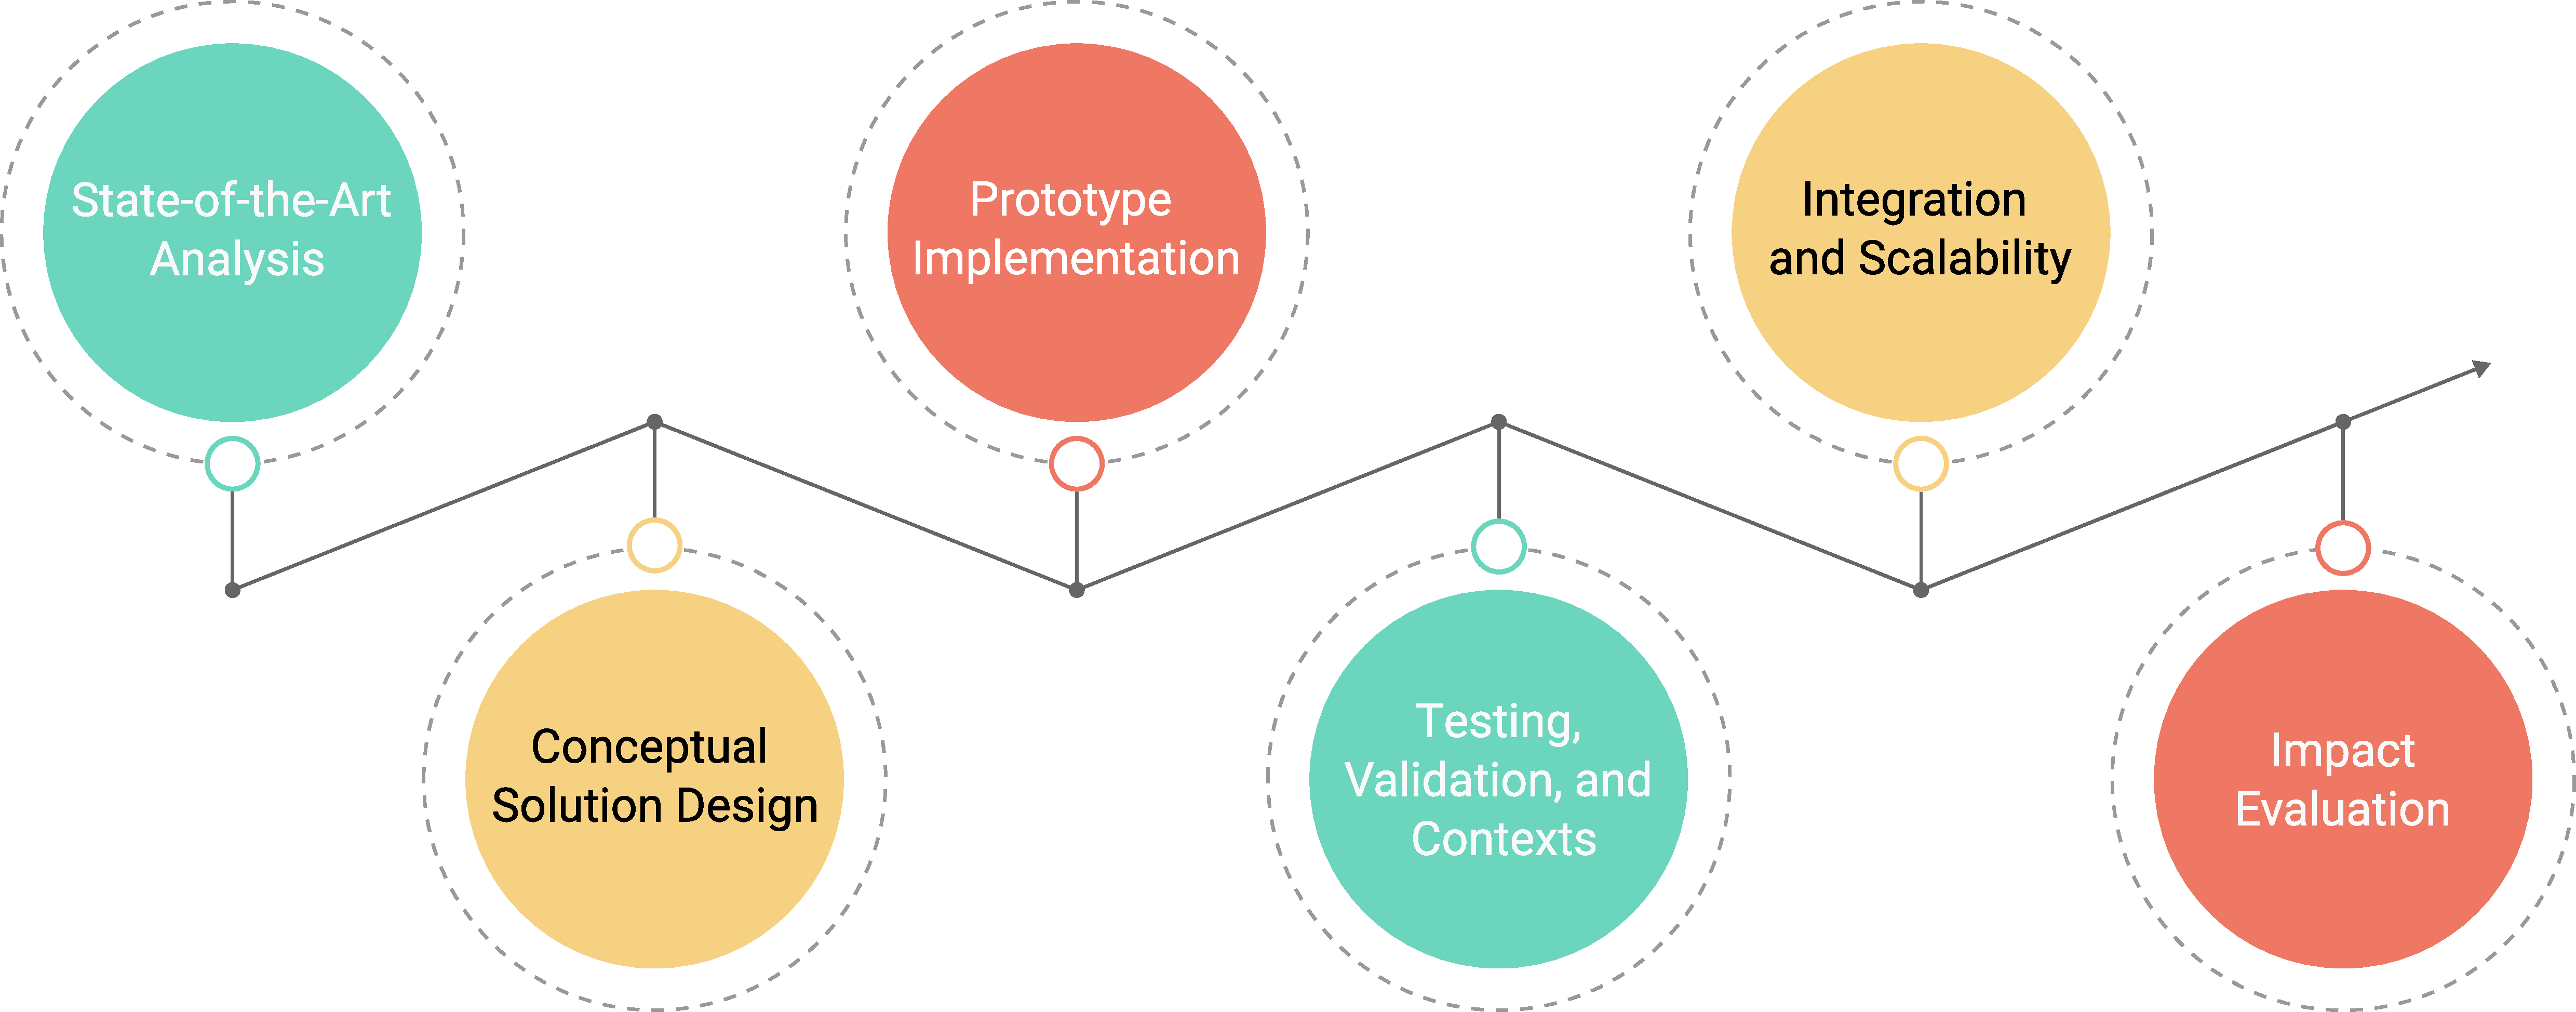
\includegraphics[width=0.8\columnwidth]{images/general_methodology}
\end{figure}
\vfill{}

\begin{center}
\textsl{\textcolor{red}{\scriptsize{}A six-step approach to analyze,
design, prototype, test, integrate, and evaluate real-time AI-driven
solutions.}}{\scriptsize\par}
\par\end{center}

\end{frame}
%
\begin{frame}{AI Hyperparameter Tuning and System-Level Optimization}

\framesubtitle{Enhancing Model Performance and System Efficiency through Dual Optimization
Techniques}
\begin{columns}[t]

\column[t]{0.5\textwidth}

\textit{\footnotesize{}Joint Optimization Approach}{\footnotesize\par}
\begin{itemize}
\item {\footnotesize{}Optimize both }\textbf{\footnotesize{}model hyperparameters}{\footnotesize{}
and }\textbf{\footnotesize{}system resources}{\footnotesize{} (CPU,
memory, latency, energy) to enhance overall performance.}{\footnotesize\par}
\end{itemize}
\begin{figure}
\centering{}
\includegraphics[width=0.6\columnwidth]{images/opt}
\end{figure}


\column[t]{0.55\textwidth}

\textit{\footnotesize{}Reinforcement Learning (RL) for Adaptive Optimization}{\footnotesize\par}
\begin{itemize}
\item \textbf{\footnotesize{}RL }{\footnotesize{}adjusts }\textbf{\footnotesize{}system
resources}{\footnotesize{} (CPU/GPU, memory, network) in real-time
to maintain efficiency under changing conditions.}{\footnotesize\par}
\end{itemize}
\begin{figure}
\centering{}
\includegraphics[width=0.6\columnwidth]{images/rl}
\end{figure}

\end{columns}

\begin{center}
\rule[0.5ex]{0.8\columnwidth}{1pt}
\par\end{center}
\begin{columns}[t]

\column[b]{0.7\textwidth}

\textit{\footnotesize{}Synergy Between Techniques}{\footnotesize\par}
\begin{itemize}
\item \textbf{\footnotesize{}Bayesian Optimization}{\footnotesize{} finds
optimal initial configurations. }{\footnotesize\par}
\item \textbf{\footnotesize{}RL}{\footnotesize{} continuously adapts configurations
to maintain }\textbf{\footnotesize{}efficiency}{\footnotesize{} under
different operational conditions.}{\footnotesize\par}
\end{itemize}

\column[b]{0.3\textwidth}

\begin{figure}
\centering{}
\includegraphics[width=0.7\columnwidth]{images/syn}
\end{figure}

\end{columns}

\begin{center}
\vfill{}
\textit{\textcolor{red}{\scriptsize{}By integrating }}\textbf{\textit{\textcolor{red}{\scriptsize{}Bayesian
optimization}}}\textit{\textcolor{red}{\scriptsize{} for initial setup
with}}\textbf{\textit{\textcolor{red}{\scriptsize{} reinforcement
learning}}}\textit{\textcolor{red}{\scriptsize{} for continuous adaptation,
the goal is to achieve }}\textbf{\textit{\textcolor{red}{\scriptsize{}robust
performance}}}\textit{\textcolor{red}{\scriptsize{} and }}\textbf{\textit{\textcolor{red}{\scriptsize{}resource
efficiency}}}\textit{\textcolor{red}{\scriptsize{} under diverse system
conditions.}}{\scriptsize\par}
\par\end{center}

\end{frame}
%
\begin{frame}{Testing Contexts of Interest}

\framesubtitle{Scenarios for Testing}
\begin{columns}[t]

\column{0.5\textwidth}

\textit{\footnotesize{}Prototipo costo-eficiente y escalable para
el monitoreo del espectro radioeléctrico en Colombia mediante radio
definido por software y aprendizaje profundo.}{\footnotesize\par}
\begin{columns}[t]

\column[c]{0.45\textwidth}
\begin{itemize}
\item {\scriptsize{}Scalability}{\scriptsize\par}
\item {\scriptsize{}Robustness }{\scriptsize\par}
\item {\scriptsize{}Low Latency}{\scriptsize\par}
\item {\scriptsize{}Reliability}{\scriptsize\par}
\end{itemize}

\column[c]{0.55\textwidth}

\begin{figure}
\centering{}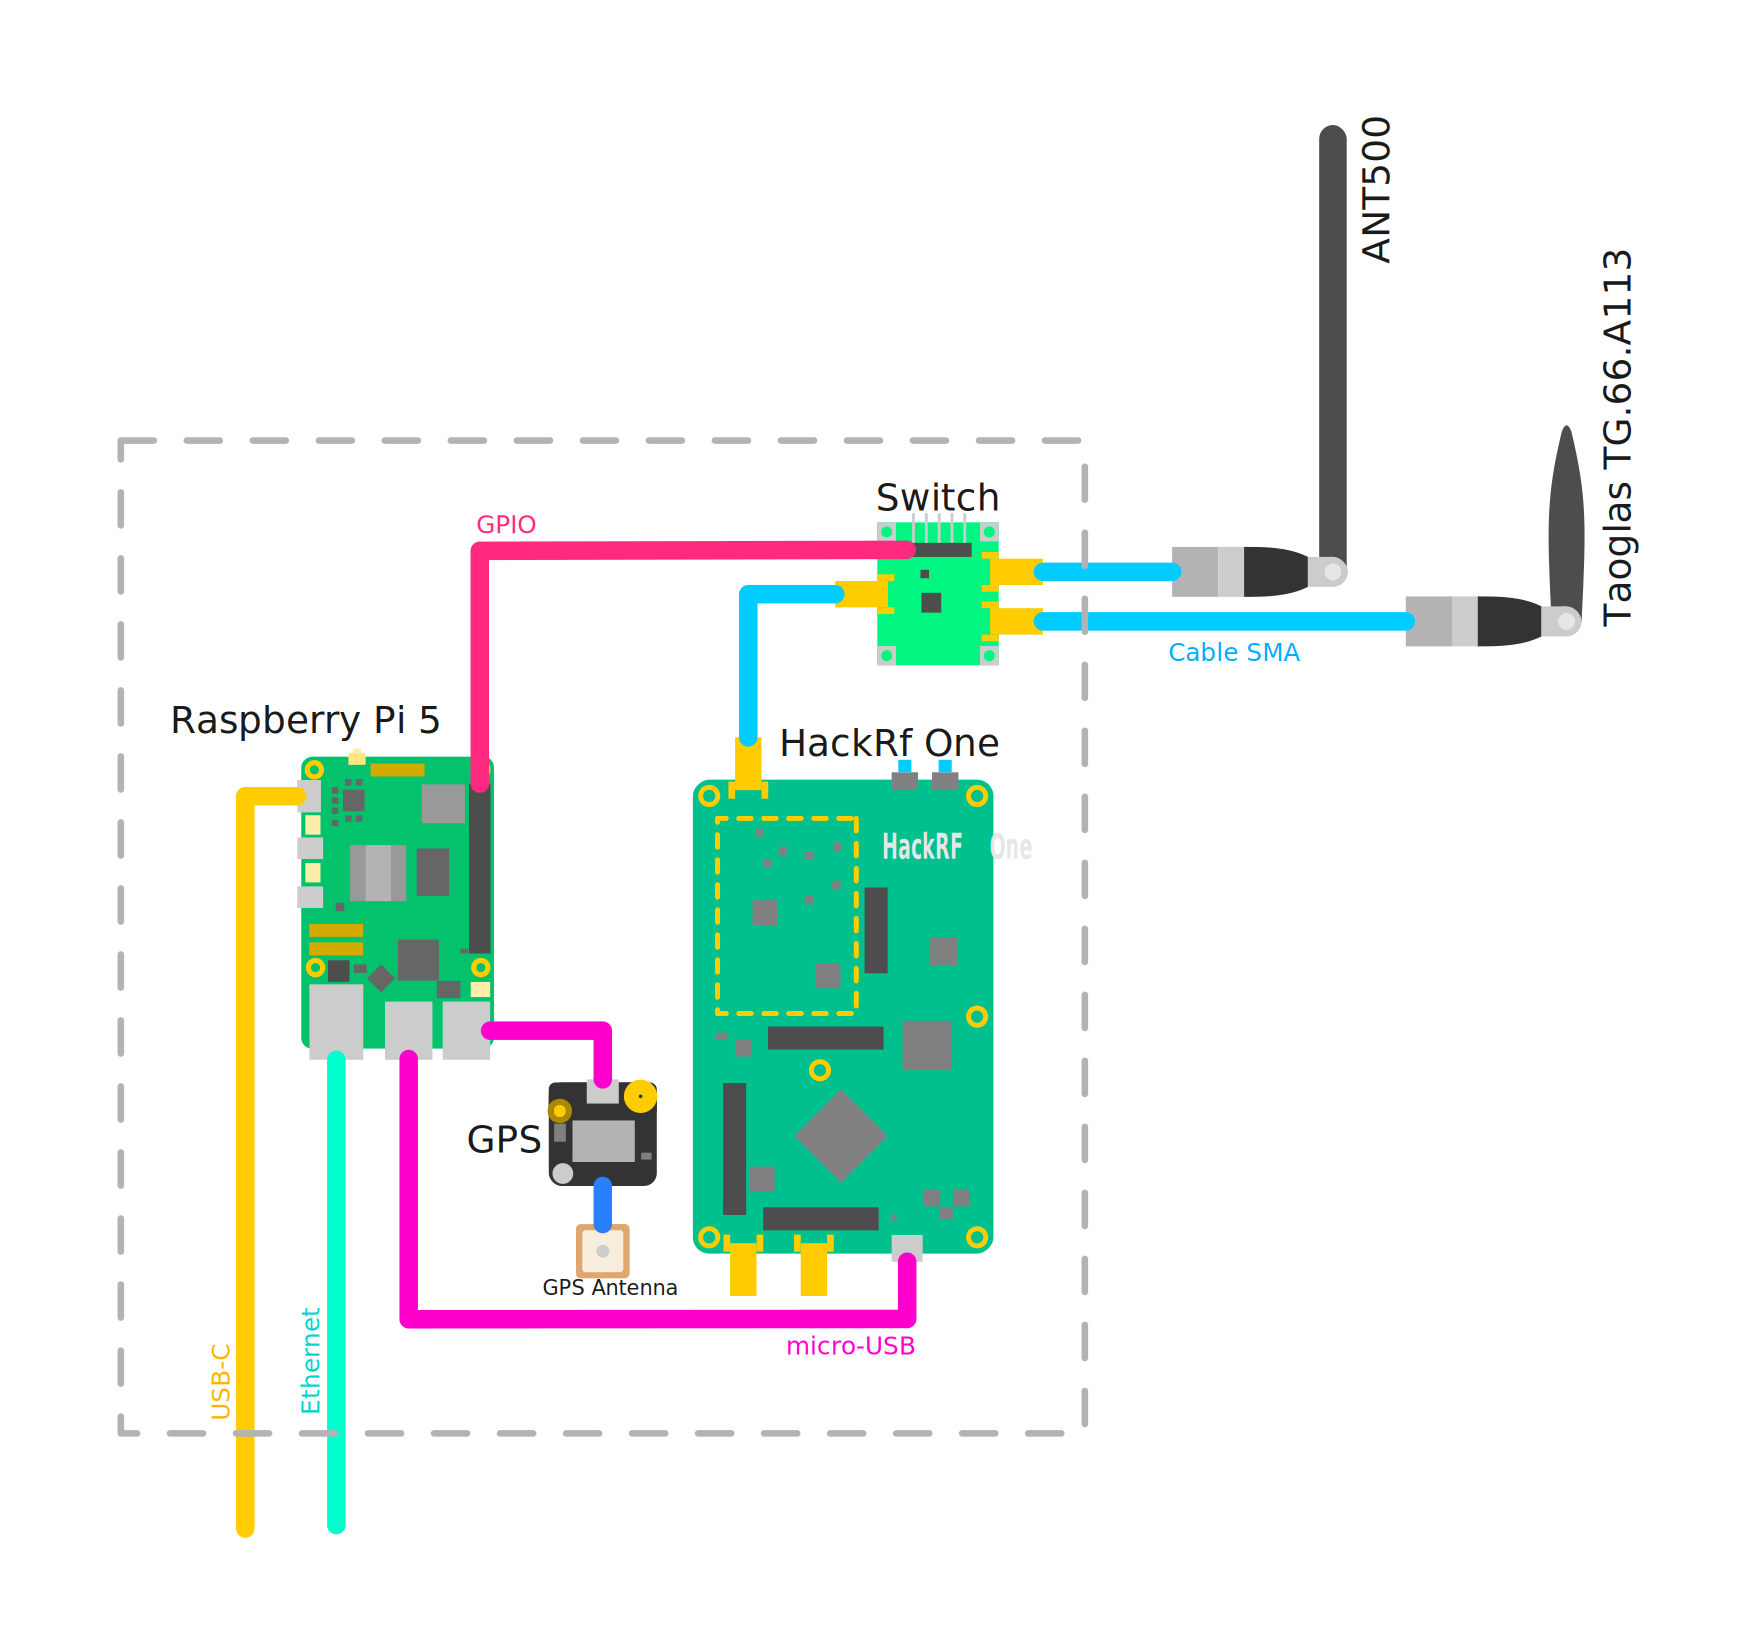
\includegraphics[height=0.4\paperheight]{images/architecture}
\end{figure}

\end{columns}

\vfill{}


\column{0.5\textwidth}

\textit{\footnotesize{}Sistema de integración de EEG, ECG y SpO2 para
seguimiento de neonatos en unidad de cuidados intensivos del Hospital
Universitario de Caldas - SES HUC.}{\footnotesize\par}
\begin{columns}[t]

\column[c]{0.5\textwidth}
\begin{itemize}
\item {\scriptsize{}Real-Time Monitoring}{\scriptsize\par}
\item {\scriptsize{}Data Centralization}{\scriptsize\par}
\item {\scriptsize{}Alarm Generation}{\scriptsize\par}
\item {\scriptsize{}Accuracy in Critical Settings}{\scriptsize\par}
\end{itemize}

\column[c]{0.5\textwidth}

\begin{figure}
\centering{}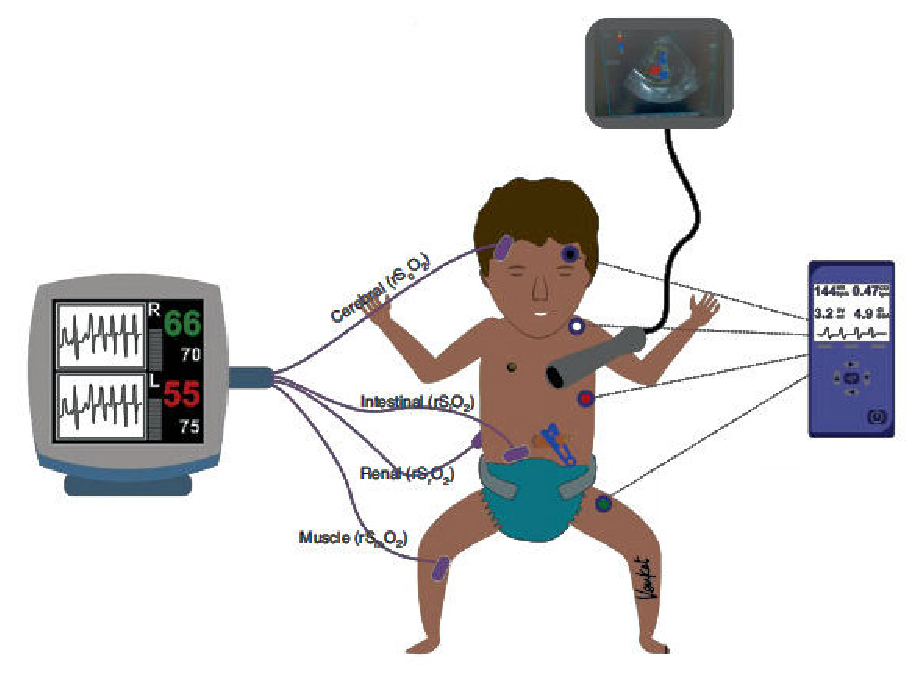
\includegraphics[width=1\columnwidth]{images/ccp}
\end{figure}

\end{columns}

\end{columns}

\begin{center}
\vfill{}
\textsl{\textcolor{red}{\scriptsize{}Two diverse research projects
provide essential testing environments for validating scalability,
robustness, and real-time data integration as part of the system development
methodology.}}{\scriptsize\par}
\par\end{center}

\end{frame}
%
\begin{frame}{Testing Contexts of Interest}

\framesubtitle{Scenarios for Testing}
\begin{columns}[t]

\column{0.5\textwidth}

\textit{\footnotesize{}Prototipo Funcional de Lengua Electrónica para
la Identificación de Sabores en Cacao Fino de Origen Colombiano}{\footnotesize\par}
\begin{columns}[t]

\column[c]{0.45\textwidth}
\begin{itemize}
\item {\scriptsize{}Flavor Profile Identification}{\scriptsize\par}
\item {\scriptsize{}Portability and Real-Time Analysis}{\scriptsize\par}
\item {\scriptsize{}Quality Validation}{\scriptsize\par}
\end{itemize}

\column[c]{0.55\textwidth}

\begin{figure}
\centering{}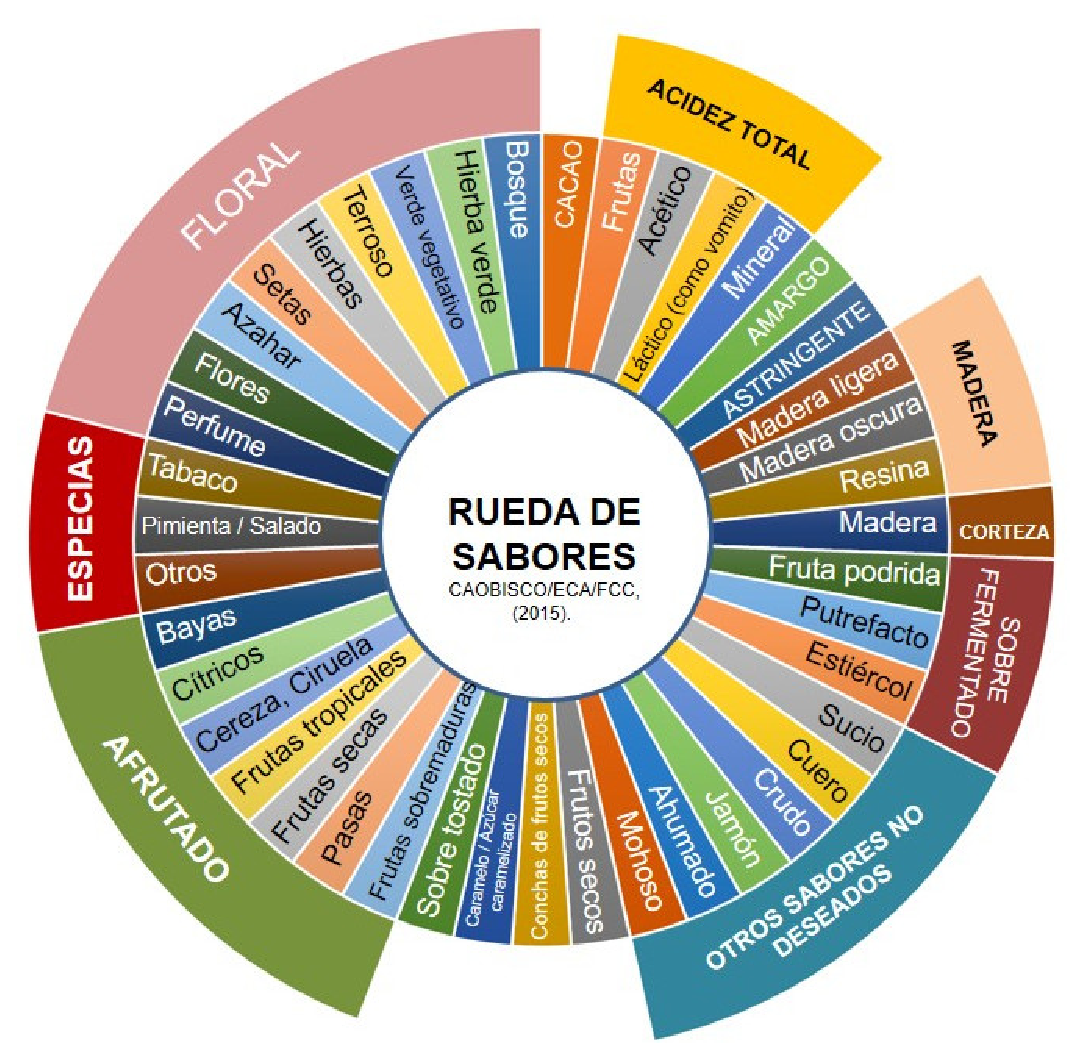
\includegraphics[width=0.75\columnwidth]{images/Rueda_Sabores}
\end{figure}

\end{columns}


\column{0.5\textwidth}

Together, these three projects provide a \textbf{comprehensive validation
of the AI-driven solution, enhancing robustness, adaptability}, and
practical applications across sectors from telecommunications to food
quality.
\end{columns}

\begin{center}
\vfill{}
\textsl{\textcolor{red}{\scriptsize{}The electronic tongue prototype
supports research by providing a practical testing environment for
enhancing flavor analysis methodologies in cacao production.}}{\scriptsize\par}
\par\end{center}

\end{frame}
%
\begin{frame}{Methodology {[}OBJ1{]}}

\framesubtitle{Streamlining Signal Integration:\\\,\,\,\,\,\,A Comprehensive
Approach to Real-Time Data Management and Visualization}
\begin{columns}[t]

\column[b]{0.4\textwidth}

\begin{figure}
\centering{}\includegraphics[width=1\columnwidth]{images/diagrams/metodology/aim1\lyxdot 1}
\end{figure}


\column[b]{0.6\textwidth}

\begin{figure}
\centering{}\includegraphics[width=1\columnwidth]{images/diagrams/metodology/aim1\lyxdot 2}
\end{figure}

\vfill{}
\end{columns}

\begin{center}
\textsl{\textcolor{red}{\scriptsize{}Create a }}\textbf{\textsl{\textcolor{red}{\scriptsize{}modular
and parameterized}}}\textsl{\textcolor{red}{\scriptsize{} system for
real-time signal acquisition, processing, and integration.}}{\scriptsize\par}
\par\end{center}

\end{frame}
%
\begin{frame}{Methodology {[}OBJ1{]}}

\framesubtitle{BCI-Framework 1.0}
\begin{columns}[t]

\column[b]{0.5\textwidth}

\begin{figure}
\centering{}\includegraphics[width=0.7\columnwidth]{images/animation/plot}
\end{figure}
\begin{figure}
\centering{}\includegraphics[width=0.7\columnwidth]{images/animation/ide}
\end{figure}


\column[b]{0.5\textwidth}

\begin{figure}
\centering{}\includegraphics[width=0.7\columnwidth]{images/animation/delivery}
\end{figure}
\begin{figure}
\centering{}\includegraphics[width=0.7\columnwidth]{images/animation/connect}
\end{figure}

\end{columns}

\begin{description}
\item [{{\scriptsize{}GitHub:}}] {\scriptsize{}\href{https://github.com/UN-GCPDS/bci-framework}{https://github.com/UN-GCPDS/bci-framework}}{\scriptsize\par}
\item [{{\scriptsize{}Documentation:}}] {\scriptsize{}\href{https://bci-framework.readthedocs.io/en/latest/}{https://bci-framework.readthedocs.io/en/latest/}}{\scriptsize\par}
\end{description}
\end{frame}
%
\begin{frame}{Methodology {[}OBJ2{]}}

\framesubtitle{Optimizing System Performance: Configuring Key Parameters for Enhanced
Efficiency and Security}

\begin{columns}[t]

\column[b]{0.5\textwidth}

\begin{figure}
\centering{}\includegraphics[width=1\columnwidth]{images/diagrams/metodology/aim2\lyxdot 1}
\end{figure}
\vfill{}

\begin{center}
\textsl{\textcolor{red}{\scriptsize{}Implement }}\textbf{\textsl{\textcolor{red}{\scriptsize{}AI-driven
automation}}}\textsl{\textcolor{red}{\scriptsize{} for optimizing
real-time API and ETL configurations.}}{\scriptsize\par}
\par\end{center}

\column[b]{0.5\textwidth}

\begin{figure}
\centering{}\includegraphics[width=0.95\columnwidth]{images/diagrams/metodology/aim2\lyxdot 2}
\end{figure}

\end{columns}

\end{frame}
%
\begin{frame}{Methodology {[}OBJ2{]}}

\framesubtitle{Scalable Service Management for AI Applications}

\textbf{Foundation} is a scalable AI framework for managing distributed
services and data processes, designed to optimize efficiency and flexibility
in Docker Swarm environments.
\begin{columns}[t]

\column[b]{0.77\textwidth}
\begin{itemize}
\item \textbf{\scriptsize{}Service Management:}{\scriptsize{} Automates
creation, deletion, and scaling of services in Docker Swarm. }{\scriptsize\par}
\item \textbf{\scriptsize{}Worker Lifecycle Control:}{\scriptsize{} Manages
Python, Django, and Brython services, ensuring efficient deployment
and operation. }{\scriptsize\par}
\item \textbf{\scriptsize{}Distributed Logging:}{\scriptsize{} Centralized
log management via HTTP and Kafka for better monitoring. }{\scriptsize\par}
\item \textbf{\scriptsize{}Dynamic Resource Allocation:}{\scriptsize{} Adaptive
management of CPU, memory, and network resources to optimize performance.}{\scriptsize\par}
\item \textbf{\scriptsize{}Integration with AI Models:}{\scriptsize{} Supports
integration of machine learning models for automated decision-making
and optimization.}{\scriptsize\par}
\end{itemize}

\column[b]{0.15\textwidth}

\begin{figure}
\centering{}\includegraphics[width=1\columnwidth]{images/diagrams/metodology/foundation}
\end{figure}

\end{columns}

\vfill{}

\begin{description}
\item [{{\scriptsize{}GitHub:}}] {\scriptsize{}\href{https://github.com/dunderlab/python-dunerlab.foundation}{https://github.com/dunderlab/python-dunerlab.foundation}}{\scriptsize\par}
\item [{{\scriptsize{}Documentation:}}] {\scriptsize{}\href{https://dunderlab-foundation.readthedocs.io/en/latest/index.html}{https://dunderlab-foundation.readthedocs.io/en/latest/index.html}
(Not yet)}{\scriptsize\par}
\end{description}
\end{frame}
%
\begin{frame}{Methodology {[}OBJ3{]}}

\framesubtitle{Building Advanced AI-based Network protocols: Enhancing Communication
and Data Transfer Efficiency}

\begin{columns}[t]

\column[b]{0.5\textwidth}

\begin{figure}
\centering{}\includegraphics[width=1\columnwidth]{images/diagrams/metodology/aim3\lyxdot 1}
\end{figure}


\column[b]{0.5\textwidth}

\begin{figure}
\centering{}\includegraphics[width=1\columnwidth]{images/diagrams/metodology/aim3\lyxdot 2}
\end{figure}
\vfill{}

\end{columns}

\begin{center}
\textsl{\textcolor{red}{\scriptsize{}Build a scalable, }}\textbf{\textsl{\textcolor{red}{\scriptsize{}AI-enhanced
platform}}}\textsl{\textcolor{red}{\scriptsize{} for efficient file
transmission and distributed messaging.}}{\scriptsize\par}
\par\end{center}

\end{frame}
%
\begin{frame}{Methodology {[}OBJ3{]}}

\framesubtitle{Dynamic Communication Framework for Distributed Networks}

\textbf{Chaski-Confluent} is a distributed communication framework
designed for scalable message handling and dynamic node pairing, tailored
for TCP/IP networks and optimized for efficient data exchange.
\begin{columns}[t]

\column[b]{0.75\textwidth}
\begin{itemize}
\item \textbf{\scriptsize{}Scalable Messaging:}{\scriptsize{} Supports robust
node discovery and efficient message routing in large-scale networks. }{\scriptsize\par}
\item \textbf{\scriptsize{}Dynamic Node Pairing:}{\scriptsize{} Manages
automatic pairing of nodes based on subscription topics, ensuring
adaptive communication. }{\scriptsize\par}
\item \textbf{\scriptsize{}Remote Python Execution:}{\scriptsize{} Facilitates
remote Python script execution similar to RPyC, enhancing computational
flexibility. }{\scriptsize\par}
\item \textbf{\scriptsize{}AI-Enhanced Data Transfer:}{\scriptsize{} Integrates
AI-based techniques for optimizing large file transfers and message
distribution. }{\scriptsize\par}
\item \textbf{\scriptsize{}Real-Time Adaptability:}{\scriptsize{} Adjusts
to network changes for improved communication and resource utilization.}{\scriptsize\par}
\end{itemize}

\column[b]{0.2\textwidth}

\begin{figure}
\centering{}\includegraphics[width=1\columnwidth]{images/diagrams/metodology/chaski}
\end{figure}

\end{columns}

\vfill{}

\begin{description}
\item [{{\scriptsize{}GitHub:}}] {\scriptsize{}\href{https://github.com/dunderlab/python-chaski}{https://github.com/dunderlab/python-chaski}}{\scriptsize\par}
\item [{{\scriptsize{}Documentation:}}] {\scriptsize{}\href{https://chaski-confluent.readthedocs.io/en/latest/}{https://chaski-confluent.readthedocs.io/en/latest/}}{\scriptsize\par}
\end{description}
\end{frame}

\section{Obtained Results}
\begin{frame}{Obtained Results}

\framesubtitle{Papers}
\begin{description}
\item [{{\scriptsize{}{[}2023{]}}}] \noindent {\scriptsize{}Published a
research paper titled \textquotedbl}\textbf{\scriptsize{}A Novel
OpenBCI Framework for EEG-Based Neurophysiological Experiments}{\scriptsize{}\textquotedbl{}
in the journal Sensors. The paper discusses the development of an
Open Brain-Computer Interface (OpenBCI) framework, utilizing open-source
hardware and firmware to facilitate EEG-based neurophysiological experiments.
The framework is designed to overcome the limitations of OpenBCI systems,
particularly in communication and flexibility for various neurophysiological
protocols. The research was published in Volume 23, Issue 7 of Sensors,
2023 (DOI: 10.3390/s23073763) (MDPI).}{\footnotesize{}\vfill{}
}{\footnotesize\par}
\item [{{\scriptsize{}{[}2023{]}}}] {\scriptsize{}At the \textquotedbl III
Congreso Latinoamericano de Investigación, Innovación y Emprendimiento
Educativo,\textquotedbl{} presented \textquotedbl}\textbf{\scriptsize{}Real-Time
Processing for BCI-Based MI Paradigms Using Deep Learning Models}{\scriptsize{}\textquotedbl{}
This paper showcases advancements in BCI technology, highlighting
the application of deep learning models for efficient, real-time processing
in Motor Imagery (MI) paradigms. The study emphasizes improvements
in processing speed and accuracy, addressing challenges in real-time
applications and setting new standards for BCI system performance.
The work has significant implications for both academic research and
practical BCI applications in various fields.}{\scriptsize\par}
\end{description}
\end{frame}
%
\begin{frame}{Obtained Results}

\framesubtitle{Patents and software registers}
\begin{description}
\item [{{\scriptsize{}{[}2022{]}}}] \noindent {\scriptsize{}The systems
were submitted to the Crearlo no es suficiente summons for a patentability
search process with the Universidad Nacional de Colombia sede Manizales
as main beneficiary with the title \textquotedbl}\textbf{\scriptsize{}MÉTODO
Y SISTEMA PARA LA SINCRONIZACIÓN DE MARCADORES ASOCIADOS A SISTEMAS
DE INTERFAZ CEREBRO-COMPUTADOR}{\scriptsize{}\textquotedbl , postulation
ID 343 and Application number NC2022/0007405 from May 28, 2022.}{\footnotesize{}\vfill{}
}{\footnotesize\par}
\item [{{\scriptsize{}{[}2022{]}}}] \noindent {\scriptsize{}A script developed
with BCI-Framework for}\textbf{\scriptsize{} Motor imagery paradigm
with game-based stimulus (Pacman interface)}{\scriptsize{} was submitted
to the software register in the Universidad Nacional de Colombia sede
Manizales.}{\scriptsize\par}
\end{description}
\end{frame}
%


\section{Implementation Schedule}
\begin{frame}{Implementation Schedule}

\centering \scalebox{0.8}{

\begin{table}[] \scriptsize \begin{tabular}{c|lllllllllllllllllllllllllll|}                          & \multicolumn{27}{c|}{Activities}                                                                                                                                                                                                                                                                                                                                                                                                                                                                                                                                                                                                                                                                                                                                                                                            \\ \cline{2-28}                           & \multicolumn{7}{c|}{}                                                                                                                                                                                           & \multicolumn{7}{c|}{}                                                                                                                                                                                           & \multicolumn{9}{c|}{}                                                                                                                                                                                                                                                 & \multicolumn{4}{c|}{\begin{tabular}[c]{@{}c@{}}Papers and thesis \\ document writing\end{tabular}}              \\ \cline{25-28}  \multirow{-2}{*}{Months} & \multicolumn{7}{c|}{\multirow{-2}{*}{Phases OBJ 1}}                                                                                                                                                             & \multicolumn{7}{c|}{\multirow{-2}{*}{Phases OBJ 2}}                                                                                                                                                             & \multicolumn{9}{c|}{\multirow{-2}{*}{Phases OBJ 3}}                                                                                                                                                                                                                   & \multicolumn{1}{l|}{Paper} & \multicolumn{1}{l|}{Paper} & \multicolumn{1}{l|}{Paper} & Thesis                   \\ \hline 1-2                      & \cellcolor[HTML]{BED189} &                          &                          &                          &                          &                          & \multicolumn{1}{l|}{}                         & \cellcolor[HTML]{BED189} &                          &                          &                          &                          &                          & \multicolumn{1}{l|}{}                         & \cellcolor[HTML]{BED189} &                          &                          &                          &                          &                          &                          &                          & \multicolumn{1}{l|}{}                         &                            &                            &                            &                          \\ 2-4                      &                          & \cellcolor[HTML]{BED189} &                          &                          &                          &                          & \multicolumn{1}{l|}{}                         &                          & \cellcolor[HTML]{BED189} &                          &                          &                          &                          & \multicolumn{1}{l|}{}                         &                          & \cellcolor[HTML]{BED189} &                          &                          &                          &                          &                          &                          & \multicolumn{1}{l|}{}                         &                            &                            &                            &                          \\ 4-6                      &                          &                          & \cellcolor[HTML]{BED189} & \cellcolor[HTML]{BED189} &                          &                          & \multicolumn{1}{l|}{}                         &                          &                          &                          &                          &                          &                          & \multicolumn{1}{l|}{}                         &                          &                          &                          &                          &                          &                          &                          &                          & \multicolumn{1}{l|}{}                         & \cellcolor[HTML]{BED189}   &                            &                            & \cellcolor[HTML]{BED189} \\ 6-8                      &                          &                          &                          & \cellcolor[HTML]{BED189} & \cellcolor[HTML]{BED189} &                          & \multicolumn{1}{l|}{}                         &                          &                          &                          &                          &                          &                          & \multicolumn{1}{l|}{}                         &                          &                          &                          &                          &                          &                          &                          &                          & \multicolumn{1}{l|}{}                         & \cellcolor[HTML]{BED189}   &                            &                            & \cellcolor[HTML]{BED189} \\ 8-10                     &                          &                          &                          &                          &                          &                          & \multicolumn{1}{l|}{}                         &                          &                          & \cellcolor[HTML]{BED189} & \cellcolor[HTML]{BED189} & \cellcolor[HTML]{BED189} &                          & \multicolumn{1}{l|}{}                         &                          &                          &                          &                          &                          &                          &                          &                          & \multicolumn{1}{l|}{}                         & \cellcolor[HTML]{BED189}   & \cellcolor[HTML]{BED189}   &                            & \cellcolor[HTML]{BED189} \\ 10-12                    &                          &                          &                          &                          &                          &                          & \multicolumn{1}{l|}{}                         &                          &                          &                          & \cellcolor[HTML]{BED189} & \cellcolor[HTML]{BED189} & \cellcolor[HTML]{BED189} & \multicolumn{1}{l|}{}                         &                          &                          &                          &                          &                          &                          &                          &                          & \multicolumn{1}{l|}{}                         & \cellcolor[HTML]{BED189}   & \cellcolor[HTML]{BED189}   &                            & \cellcolor[HTML]{BED189} \\ 12-14                    &                          &                          &                          &                          &                          &                          & \multicolumn{1}{l|}{}                         &                          &                          &                          &                          &                          &                          & \multicolumn{1}{l|}{}                         &                          &                          & \cellcolor[HTML]{BED189} & \cellcolor[HTML]{BED189} & \cellcolor[HTML]{BED189} & \cellcolor[HTML]{BED189} &                          &                          & \multicolumn{1}{l|}{}                         & \cellcolor[HTML]{BED189}   & \cellcolor[HTML]{BED189}   & \cellcolor[HTML]{BED189}   & \cellcolor[HTML]{BED189} \\ 14-16                    &                          &                          &                          &                          &                          &                          & \multicolumn{1}{l|}{}                         &                          &                          &                          &                          &                          &                          & \multicolumn{1}{l|}{}                         &                          &                          &                          & \cellcolor[HTML]{BED189} & \cellcolor[HTML]{BED189} & \cellcolor[HTML]{BED189} & \cellcolor[HTML]{BED189} &                          & \multicolumn{1}{l|}{}                         & \cellcolor[HTML]{BED189}   & \cellcolor[HTML]{BED189}   & \cellcolor[HTML]{BED189}   & \cellcolor[HTML]{BED189} \\ 16-18                    &                          &                          &                          &                          &                          & \cellcolor[HTML]{BED189} & \multicolumn{1}{l|}{\cellcolor[HTML]{BED189}} &                          &                          &                          &                          &                          &                          & \multicolumn{1}{l|}{\cellcolor[HTML]{BED189}} &                          &                          &                          &                          &                          &                          &                          & \cellcolor[HTML]{BED189} & \multicolumn{1}{l|}{\cellcolor[HTML]{BED189}} & \cellcolor[HTML]{BED189}   & \cellcolor[HTML]{BED189}   & \cellcolor[HTML]{BED189}   & \cellcolor[HTML]{BED189} \\ \hline \end{tabular} \end{table}

}

\end{frame}

\section{Acknowledgements}
\begin{frame}{Acknowledgements}

This research would not have been possible without the support provided
by the project \textit{Prototipo Funcional de Lengua Electrónica para
la Identificación de Sabores en Cacao Fino de Origen Colombiano (código
202010039703)} funded by \textbf{Casa Luker}.
\end{frame}

\section{References}
\begin{frame}[allowframebreaks]{References}

{\tiny{}\bibliographystyle{apalike}
\bibliography{references}
}{\tiny\par}

\end{frame}

\end{document}
